\section{Interface}

At a high-level, the IOMMU exposes two interfaces. The CPU interface is for the
configuration and control of the IOMMU by the CPUs. The bus interface is for interacting
with the bus controllers. The bus interface accepts \textit{translation requests} and
returns translated addresses or faults.

\subsection{CPU Interface}

There are two 4K-aligned MMIO regions (the sizes are to be decided), one for accessing
translation-related register, called the \textit{register MMIO range}. The other is meant
for controlling the runtime behavior of the IOMMU, called the \textit{command MMIO range}.

The rationale of this divided regions is that some registers ('data registers') contain
data that the IOMMU utilize to carry out its function, mainly address translation.
Meanwhile, other registers ('control registers') act as 'triggers' in the sense that they
do not provide runtime data, instead they initiate certain operations of the IOMMU. This
separation facilitates the emulation of the IOMMU, so that the data registers can be
emulated by memory, which the control registers can be emulated by exceptions.

\subsubsection{Feature Discovery}

The IOMMU provides a register called \iommucap\ to allow harts to discover implemented
IOMMU features. The following bits are defined.

\begin{enumerate}
    \item S  bit: if S = 1, stage-two translation is implemented.
\end{enumerate}

\subsubsection{Feature Enable / Disable}

The IOMMU provides a register called \iommucapen\ to allow harts to enable or disable
certain features. The following bits are defined.

\begin{enumerate}
    \item E bit: if E = 1, the IOMMU is active. If E = 0, the IOMMU is inactive, all
        addresses in the memory requests are treated as physical addresses.
\end{enumerate}

\subsection{Bus Interface}

The underlying physical link with the peripheral bus that the IOMMU is working with is
\textit{implementation defined}. This link usually specifies the topology, command
interface and transport protocol with respect to utilizing the translation service of
the IOMMU.

An example is that for an on-chip AXI bus, the IOMMU sits between the bus masters and the
system interconnect, and by default translate all DMA requests from devices on the bus.

The IOMMU manages address translation on a per-device basis. For each device, the system
software can choose to setup address translation or configure it to be in the bypass mode
that directly works with physical addresses. 

The devices' memory accesses are treated as a sequence of transactions. Each transaction
may contain more than one transfer operation on the bus. The IOMMU works with
transactions, considering all addresses and data transferred within one transaction as a
whole group.

The IOMMU expects that the address range in the transactions adheres to restrictions
imposed by the bus protocol of that device. Typically, such restrictions limit the range
to within a 4K-aligned range, which is the minimum page size supported by the IOMMU. The
IOMMU does not perform more than one translation for each memory transaction. When the
IOMMU receives a transaction whose address range exceeds such limitation, it signals
failure to the device immediately.
% This limitation can be alleviated by using larger page sizes. %

The IOMMU does not affect the caching and ordering part of the peripheral bus protocol, if
any.

\subsection{Components and Placement}

The architecture presented in Section \ref{sec:sys_arch} illustrates the high-level
concept of the IOMMU's role in the whole system. Actual hardware implementation does not
need to strictly follow the illustration. In fact, depending on the requirement, a system
may choose to present a view of the IOMMU configuration different from the actual hardware
implementation. For example, a system may choose to configure the devices in the following
manner: assigning one IOMMU for one device and arranging for multiple device to share
another IOMMU, as illustrated in Figure \ref{fig:cmp_plcmnt}

\begin{figure}[ht!]
    \centering
    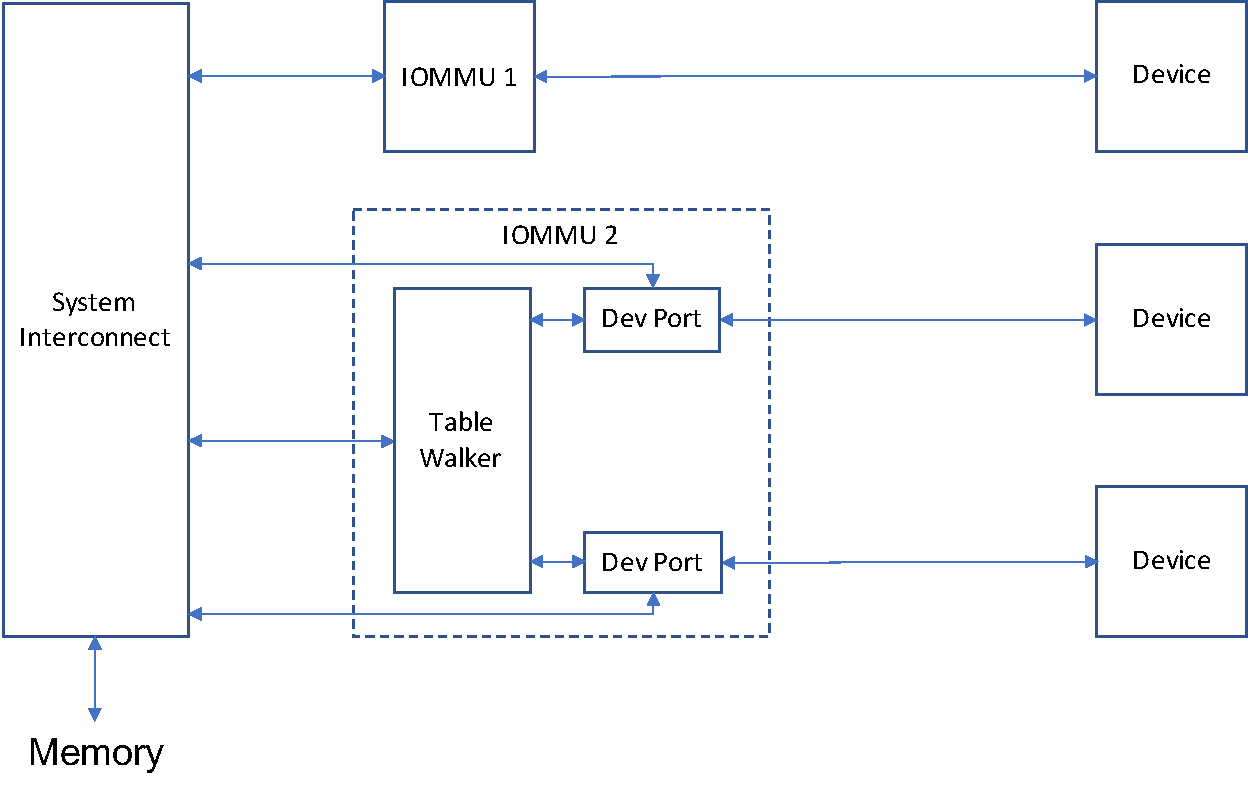
\includegraphics[width=0.95\textwidth]{img/cmp_plcmnt.pdf}
    \caption{An Example Configuration}
    \label{fig:cmp_plcmnt}
\end{figure}

However, the underlying hardware implementation can be very different. The dedicated IOMMU
may be a monolithic unit. Meanwhile, the shared IOMMU consists of sub-modules such as
device ports, translation table walker and buffers and caches. The implementation is
free to incorporate custom means to coordinate the operations of the sub-modules. However,
the components as a whole is logically exposed as one IOMMU.

It is possible for multiple IOMMU to collaborate. For example, one dedicated IOMMU may be
'dumb' and merely consists of a number of buffered translation entries. On a buffer miss,
this IOMMU requests address translation from another fully-featured IOMMU and obtains
translation results. This two IOMMUs are implemented differently, however, for some
specific reason from the platform, they are logically exposed as two functionally
equivalent IOMMU. Obviously, the necessary interaction between IOMMUs in this example is
\textit{implementation defined}. Figure \ref{fig:collab} illustrates this situation.

\begin{figure}[ht!]
    \centering
    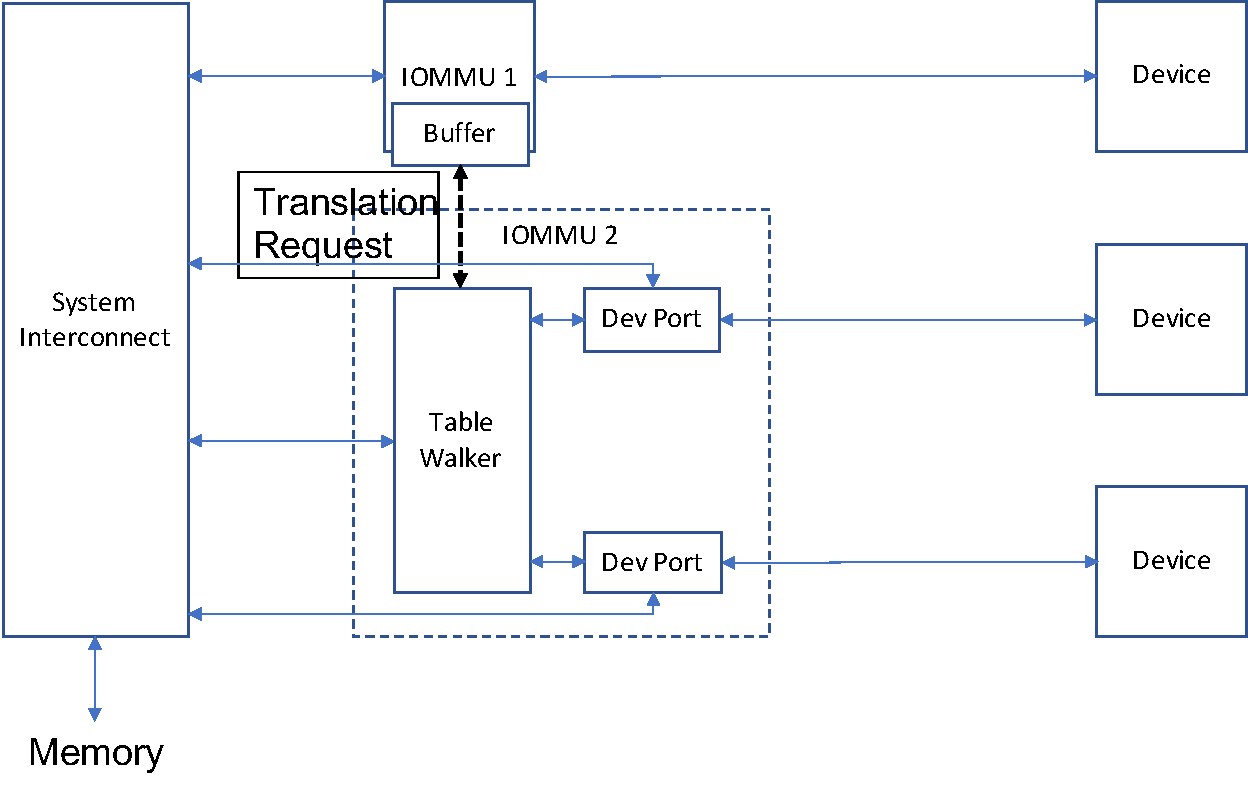
\includegraphics[width=0.95\textwidth]{img/collab.pdf}
    \caption{IOMMU Collaboration}
    \label{fig:collab}
\end{figure}



